\documentclass{beamer}
\usepackage{../../shared/styles/custom}
\usepackage{../../shared/styles/conventions}

%\beamerdefaultoverlayspecification{<+->}




\title{Coordinate Descent}
\date{\today}
\author{Nipun Batra}
\institute{IIT Gandhinagar}

\begin{document}
\maketitle


\begin{frame}{Coordinate Descent}
\begin{itemize}[<+->]
	\item Another optimisation method (akin to gradient descent)
	\item Objective: $\min_{\vtheta} f(\vtheta)$
	\item Key idea: Sometimes difficult to find minimum for all coordinates
	\item ..., but, easy for each coordinate
	\item turns into a one-dimensional optimisation problem
\end{itemize}
\end{frame}

% {
% 	\setbeamercolor{background canvas}{bg=}
% 	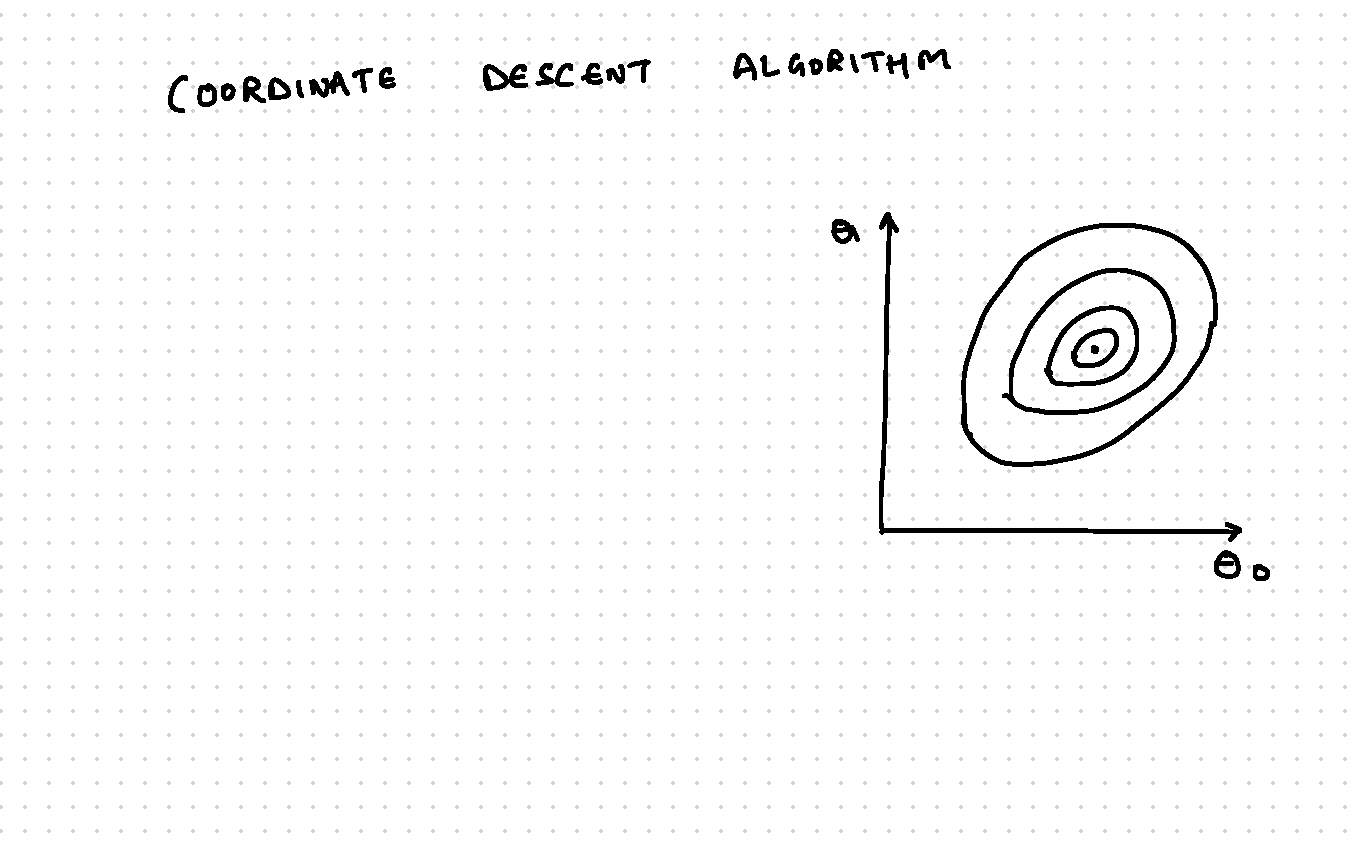
\includepdf[page=-]{../assets/coordinate-vis.pdf}
% }


\begin{frame}{Coordinate Descent}
\begin{itemize}[<+->]
	\item Picking next coordinate: \pause random, round-robin
	\item No step-size to choose!
	\item Converges for Lasso objective
\end{itemize}
\end{frame}




	\begin{frame}{Coordinate Descent : Example}
Learn $y = \theta_0 + \theta_1 x$ on following dataset, using coordinate descent where initially $(\theta_0, \theta_1) = (2,3)$ for 2 iterations. 
\begin{table}[]
	\centering
	\label{tab:my-table}
	\begin{tabular}{|c|c|}
		\hline
		\textbf{x} & \textbf{y} \\ \hline
		1 & 1 \\ \hline
		2 & 2 \\ \hline
		3 & 3 \\ \hline
	\end{tabular}
\end{table}
\end{frame}



\begin{frame}{Coordinate Descent : Example}
Our predictor, $\hat{y} = \theta_0 + \theta_1x$\\
\vspace{1cm}
Error for $i^{th}$ datapoint, $\epsilon_i = y_i - \hat{y_i}$\\
$\epsilon_1 = 1 - \theta_0 - \theta_1$ \\
$\epsilon_2 = 2 - \theta_0 - 2\theta_1$ \\
$\epsilon_3 = 3 - \theta_0 - 3\theta_1$ \\

\vspace{1cm}
MSE = $\frac{\epsilon_1^2 + \epsilon_2^2 + \epsilon_3^2}{3}$ = $\frac{14 + 3\theta_0^2 + 14\theta_1^2 -12\theta_0 - 28\theta_1 + 12\theta_0\theta_1}{3}$\\
\end{frame}





\begin{frame}{Iteration 0}

MSE = $\frac{1}{3}(14+3\theta_{0}^{2}+14\theta_{1}^{2}-12\theta_{0}-28\theta_{1}+12\theta_{0}\theta_{1})$\\

\begin{columns}
	\begin{column}{0.6\textwidth}
		\begin{adjustbox}{max totalsize={\textwidth},center}
			
			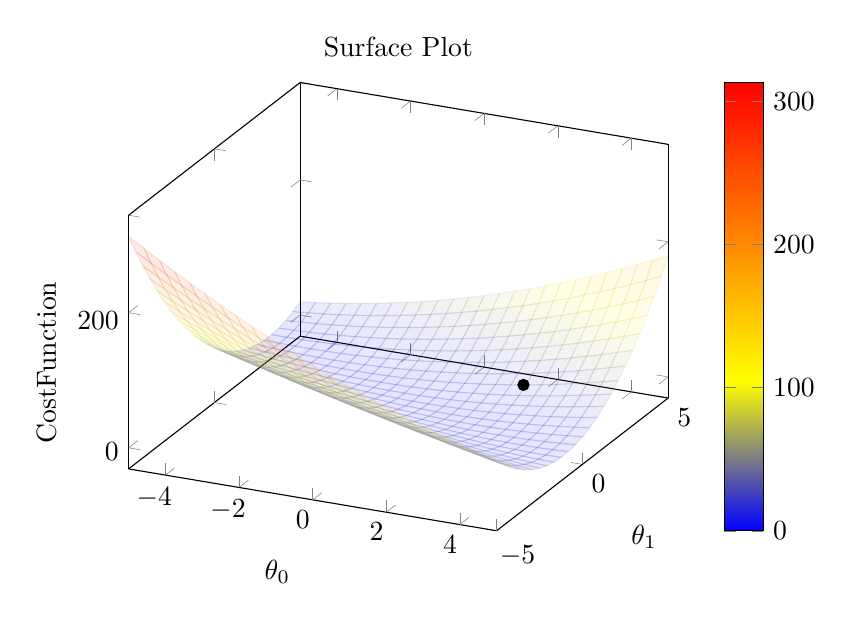
\begin{tikzpicture}
			\begin{axis}[colorbar,xlabel=$\theta_0$, ylabel=$\theta_1$, zlabel=$\mathrm{Cost Function}$,title={Surface Plot}]
			\addplot3[
			surf,opacity=0.1,
			]
			{(14 + 3*x^2 +14*y^2 -12*x - 28*y + 12*x*y)/3};
			\addplot[only marks, mark=*]
			coordinates{ % plot 1 dataset
				( 2 , 3 )
			}; 
			\end{axis}
			\end{tikzpicture}
		\end{adjustbox}
		
	\end{column}
 \begin{column}{0.5\textwidth}
		\begin{adjustbox}{max totalsize={\textwidth},center}
			\begin{tikzpicture}
			\begin{axis}
			[
			title={Contour plot, view from top},
			view={0}{90},
			xlabel=$\theta_0$,
			ylabel=$\theta_1$,
			axis x line*=bottom,
			axis y line*=left,
			xtick align=outside,
			ytick align=outside,
			unit vector ratio*=1 1 1,
			]
			\addplot3[
			contour gnuplot={number=25,}
			]
			{(14 + 3*x^2 +14*y^2 -12*x - 28*y + 12*x*y)/3};
			\addplot[only marks, mark=*]
			coordinates{ % plot 1 dataset
				( 2 , 3 )
			};
			
			
			\end{axis}
			\end{tikzpicture}
		\end{adjustbox}
	\end{column}
\end{columns}




\end{frame}

\begin{frame}{Coordinate Descent : Example}
\textbf{Iteration 1}\\
\vspace{0.5cm}
INIT: $\theta_{0} = 2$ and  $\theta_{1}  = 3$\\

\vspace{0.5cm}
$\theta_1 = 3$ optimize for $\theta_{0}$\\ 
\only<2->{
\vspace{0.5cm}
 $\frac{\partial \MSE}{\partial \theta_{0}} = 6\theta_0 + 24 = 0$\\
 \vspace{0.5cm}
 $\theta_0 = -4$


}


\end{frame}


\begin{frame}{Iteration 1}

MSE = $\frac{1}{3}(14+3\theta_{0}^{2}+14\theta_{1}^{2}-12\theta_{0}-28\theta_{1}+12\theta_{0}\theta_{1})$\\

\begin{columns}
	\begin{column}{0.6\textwidth}
		\begin{adjustbox}{max totalsize={\textwidth},center}
			
			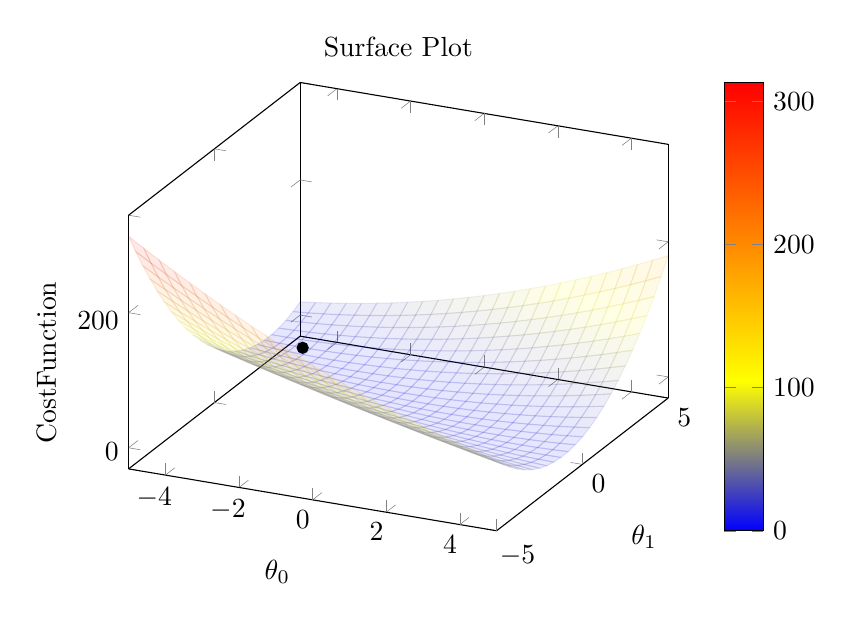
\begin{tikzpicture}
			\begin{axis}[colorbar,xlabel=$\theta_0$, ylabel=$\theta_1$, zlabel=$\mathrm{Cost Function}$,title={Surface Plot}]
			\addplot3[
			surf,opacity=0.1,
			]
			{(14 + 3*x^2 +14*y^2 -12*x - 28*y + 12*x*y)/3};
			\addplot[only marks, mark=*]
			coordinates{ % plot 1 dataset
				( -4 , 3 )
			}; 
		
			\end{axis}
			\end{tikzpicture}
		\end{adjustbox}
		
	\end{column}
 \begin{column}{0.5\textwidth}
		\begin{adjustbox}{max totalsize={\textwidth},center}
			\begin{tikzpicture}
			\begin{axis}
			[
			title={Contour plot, view from top},
			view={0}{90},
			xlabel=$\theta_0$,
			ylabel=$\theta_1$,
			axis x line*=bottom,
			axis y line*=left,
			xtick align=outside,
			ytick align=outside,
			unit vector ratio*=1 1 1,
			]
			\addplot3[
			contour gnuplot={number=25,}
			]
			{(14 + 3*x^2 +14*y^2 -12*x - 28*y + 12*x*y)/3};
			\draw [->] (axis cs: 2,3) -- (axis cs:-4,3);
			\end{axis}
			\end{tikzpicture}
		\end{adjustbox}
	\end{column}
\end{columns}


\end{frame}

\begin{frame}{Coordinate Descent : Example}
\textbf{Iteration 2}\\
\vspace{0.5cm}
INIT: $\theta_{0} = -4$ and  $\theta_{1}  = 3$\\

\vspace{0.5cm}
$\theta_0 = -4$ optimize for $\theta_{1}$\\ 
\only<2->{
\vspace{0.5cm}
 $\theta_1 = 2.7$
}


\end{frame}


\begin{frame}{Iteration 2}

MSE = $\frac{1}{3}(14+3\theta_{0}^{2}+14\theta_{1}^{2}-12\theta_{0}-28\theta_{1}+12\theta_{0}\theta_{1})$\\

\begin{columns}
	\begin{column}{0.6\textwidth}
		\begin{adjustbox}{max totalsize={\textwidth},center}
			
			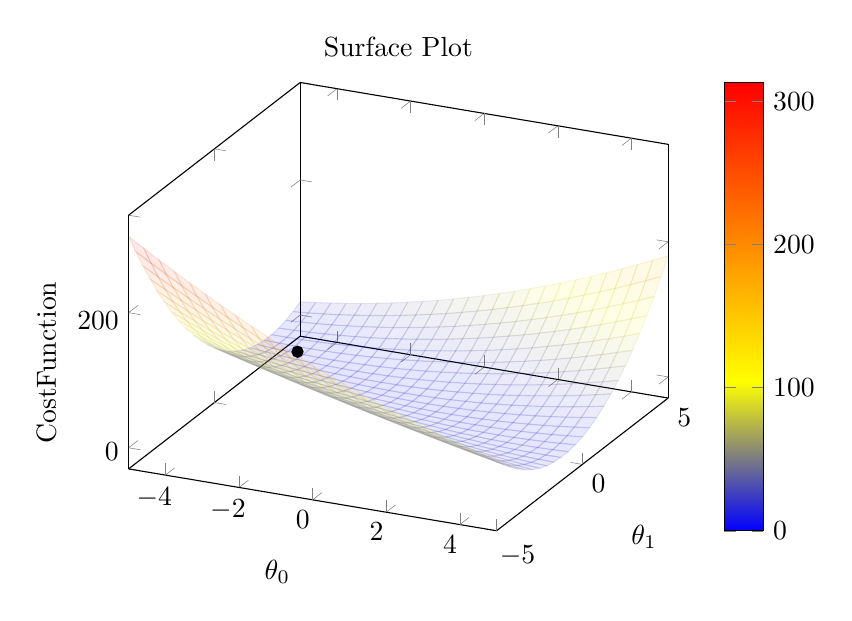
\begin{tikzpicture}
			\begin{axis}[colorbar,xlabel=$\theta_0$, ylabel=$\theta_1$, zlabel=$\mathrm{Cost Function}$,title={Surface Plot}]
			\addplot3[
			surf,opacity=0.1,
			]
			{(14 + 3*x^2 +14*y^2 -12*x - 28*y + 12*x*y)/3};
			\addplot[only marks, mark=*]
			coordinates{ % plot 1 dataset
				( -4 , 2.7 )
			}; 
	
			\end{axis}
			\end{tikzpicture}
		\end{adjustbox}
		
	\end{column}
 \begin{column}{0.5\textwidth}
		\begin{adjustbox}{max totalsize={\textwidth},center}
			\begin{tikzpicture}
			\begin{axis}
			[
			title={Contour plot, view from top},
			view={0}{90},
			xlabel=$\theta_0$,
			ylabel=$\theta_1$,
			axis x line*=bottom,
			axis y line*=left,
			xtick align=outside,
			ytick align=outside,
			unit vector ratio*=1 1 1,
			]
			\addplot3[
			contour gnuplot={number=25,}
			]
			{(14 + 3*x^2 +14*y^2 -12*x - 28*y + 12*x*y)/3};
		\draw [->] (axis cs: 2,3) -- (axis cs:-4,3);
		\draw [->] (axis cs: -4,3) -- (axis cs:-4,2.7);
			\end{axis}
			\end{tikzpicture}
		\end{adjustbox}
	\end{column}
\end{columns}


\end{frame}

\begin{frame}{Coordinate Descent : Example}
\textbf{Iteration 3}\\
\vspace{0.5cm}
INIT: $\theta_{0} = -4$ and $\theta_{1}  = 2.7$\\

\vspace{0.5cm}
$\theta_1 = 2.7$ optimize for $\theta_{0}$\\ 
\only<2->{
\vspace{0.5cm}
 $\theta_0 = -3.4$
}


\end{frame}

\begin{frame}{Iteration 3}

MSE = $\frac{1}{3}(14+3\theta_{0}^{2}+14\theta_{1}^{2}-12\theta_{0}-28\theta_{1}+12\theta_{0}\theta_{1})$\\

\begin{columns}
	\begin{column}{0.6\textwidth}
		\begin{adjustbox}{max totalsize={\textwidth},center}
			
			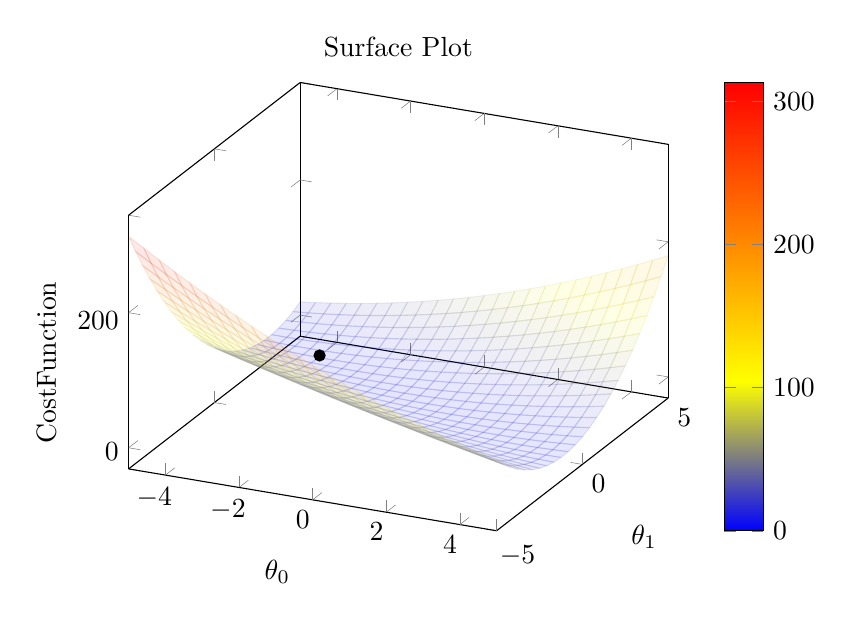
\begin{tikzpicture}
			\begin{axis}[colorbar,xlabel=$\theta_0$, ylabel=$\theta_1$, zlabel=$\mathrm{Cost Function}$,title={Surface Plot}]
			\addplot3[
			surf,opacity=0.1,
			]
			{(14 + 3*x^2 +14*y^2 -12*x - 28*y + 12*x*y)/3};
			\addplot[only marks, mark=*]
			coordinates{ % plot 1 dataset
				( -3.4 , 2.7 )
			}; 
			\end{axis}
			\end{tikzpicture}
		\end{adjustbox}
		
	\end{column}
 \begin{column}{0.5\textwidth}
		\begin{adjustbox}{max totalsize={\textwidth},center}
			\begin{tikzpicture}
			\begin{axis}
			[
			title={Contour plot, view from top},
			view={0}{90},
			xlabel=$\theta_0$,
			ylabel=$\theta_1$,
			axis x line*=bottom,
			axis y line*=left,
			xtick align=outside,
			ytick align=outside,
			unit vector ratio*=1 1 1,
			]
			\addplot3[
			contour gnuplot={number=25,}
			]
			{(14 + 3*x^2 +14*y^2 -12*x - 28*y + 12*x*y)/3};
		\draw [->] (axis cs: 2,3) -- (axis cs:-4,3);
		\draw [->] (axis cs: -4,3) -- (axis cs:-4,2.7);
		\draw [->] (axis cs: -4,2.7) -- (axis cs:-3.4,2.7);
			\end{axis}
			\end{tikzpicture}
		\end{adjustbox}
	\end{column}
\end{columns}


\end{frame}


% {
% 	\setbeamercolor{background canvas}{bg=}
% 	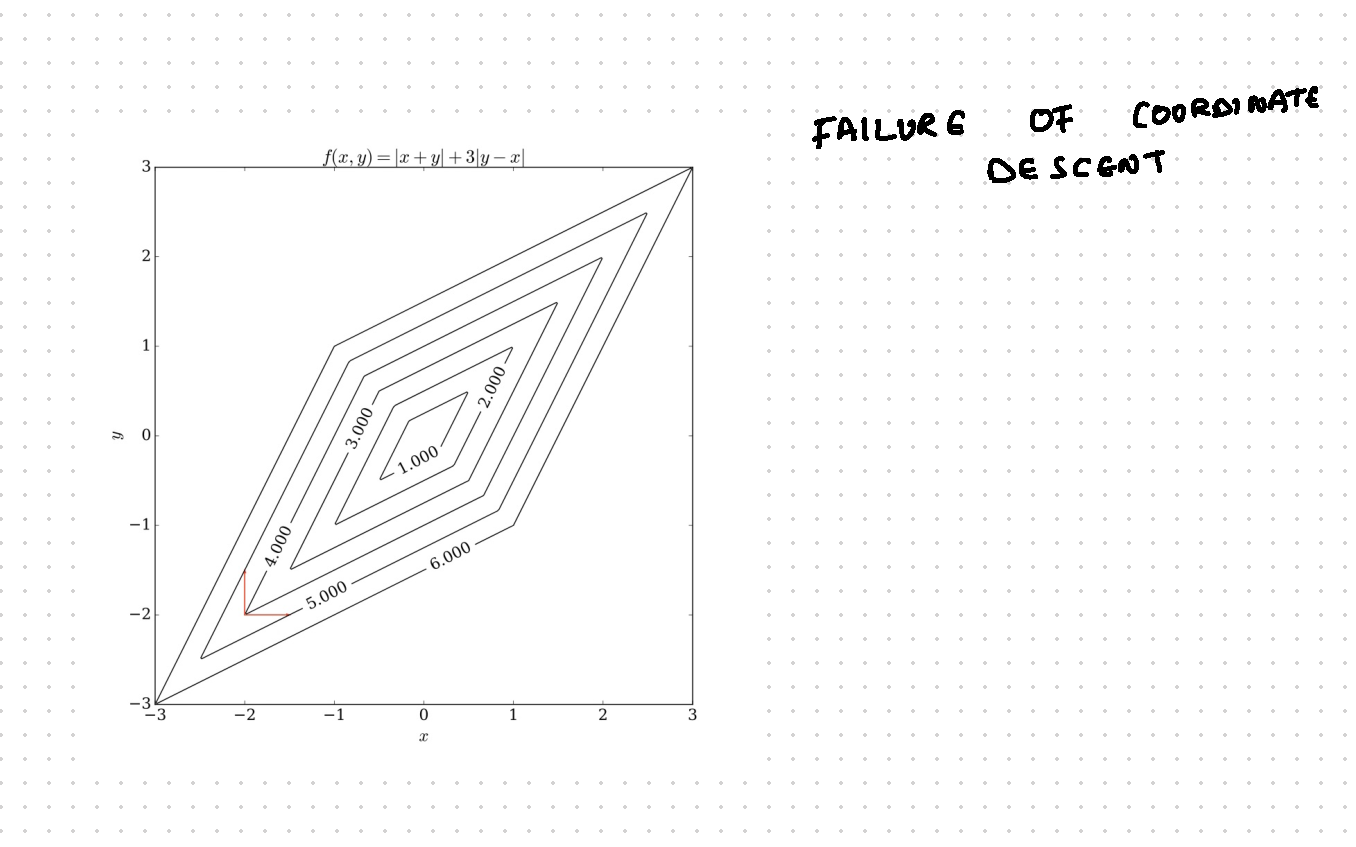
\includepdf[page=-]{../assets/coordinate-descent-fail.pdf}
% }

\end{document}
